\chapter{Testdokumentation}\label{ch:testdokumentation}
Alle Testfälle können wie beschrieben in~\enquote{\nameref{sec:testen-der-beispiele}}~ausgeführt werden.
Für eine klare Struktur wurden Sie in 4 verschiedene Testgruppen eingeteilt:
\begin{enumerate}[label={\textbf{Gruppe~\arabic*:}}, ref={Gruppe~\arabic*}, leftmargin=*, noitemsep]
    \label{enm:tesgruppen}
    \item Tests, welche die Aufgabestellung wiederspiegeln.
    \item Allgemeine Testfälle.
    \item Überprüfungen der minimal Fälle.
    \item Sonderfall Testfälle.
\end{enumerate}

Die in der Aufgabenstellung definierten Tests werden im Folgenden ausführlich beschrieben.
Dabei werden die allgemeine Funktionalität des Programms getestet.

\section{Aufgabenstellung}\label{subsec:aufgabenstellung}
\begin{figure}[!h]
    \centering
    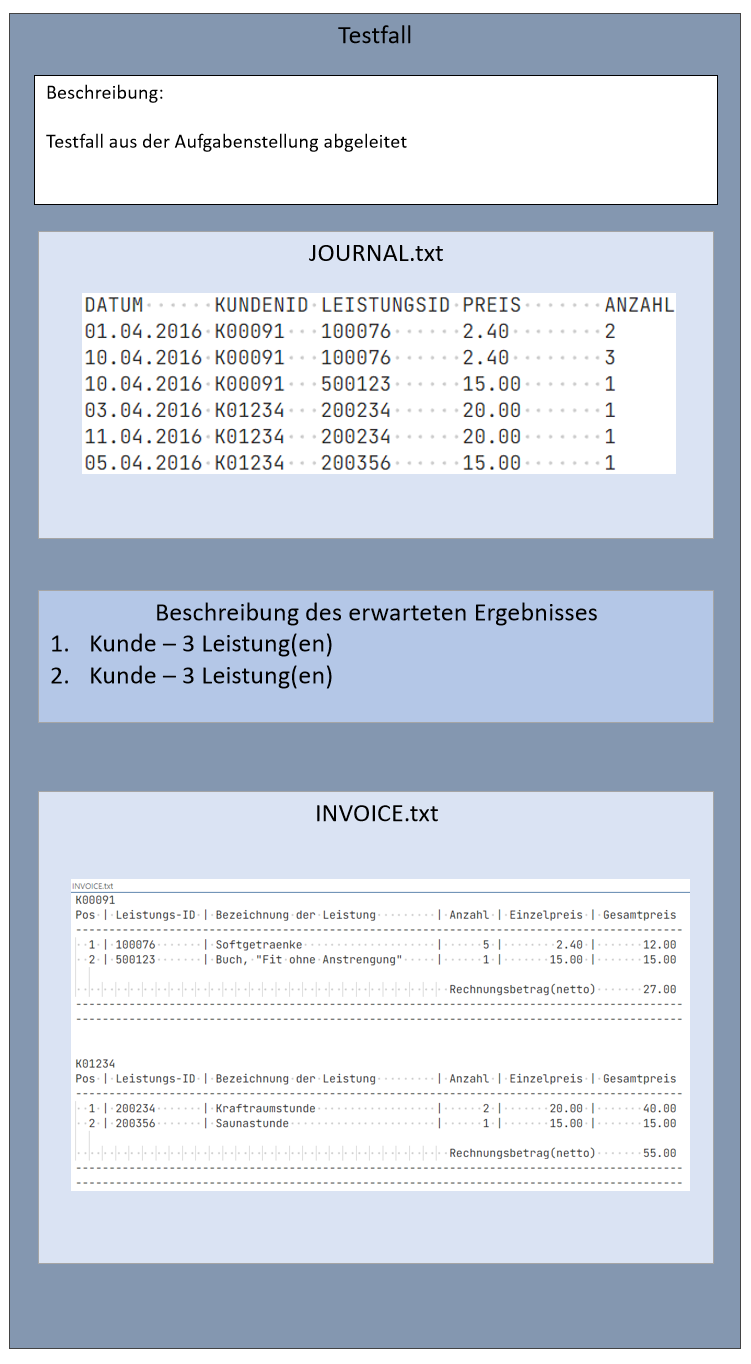
\includegraphics[width=\textwidth,height=\textheight,keepaspectratio]{images/Testdokumentation/Aufgabestellung/aufgabenstellung.png}
    \caption{Aufgabenstellung}
\end{figure}

\section{Allgemeine Tests}\label{sec:allgemeine-tests}
\begin{figure}[!h]
    \centering
    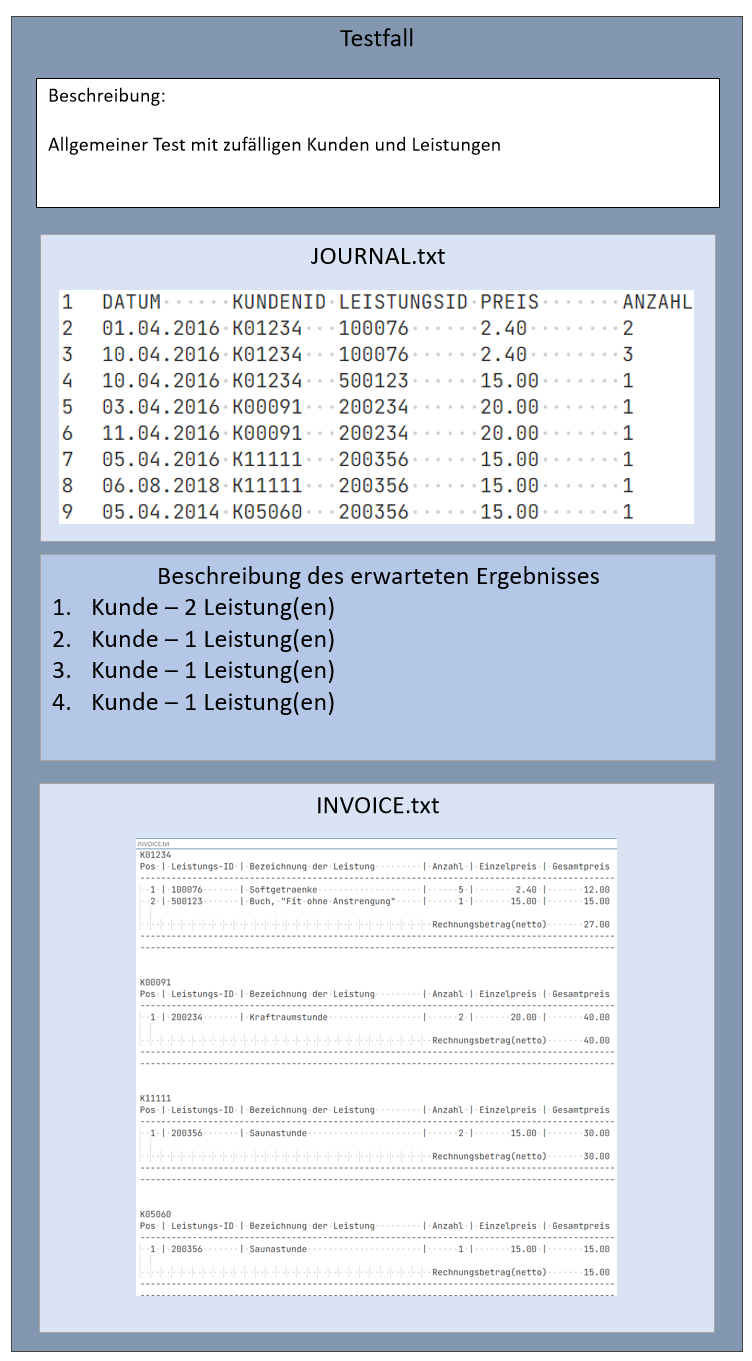
\includegraphics[width=\textwidth,height=\textheight,keepaspectratio]{images/Testdokumentation/Allgemeinfälle/fall_1.png}
    \caption{Allgemeiner Testfall 1}
\end{figure}

\begin{figure}[!h]
    \centering
    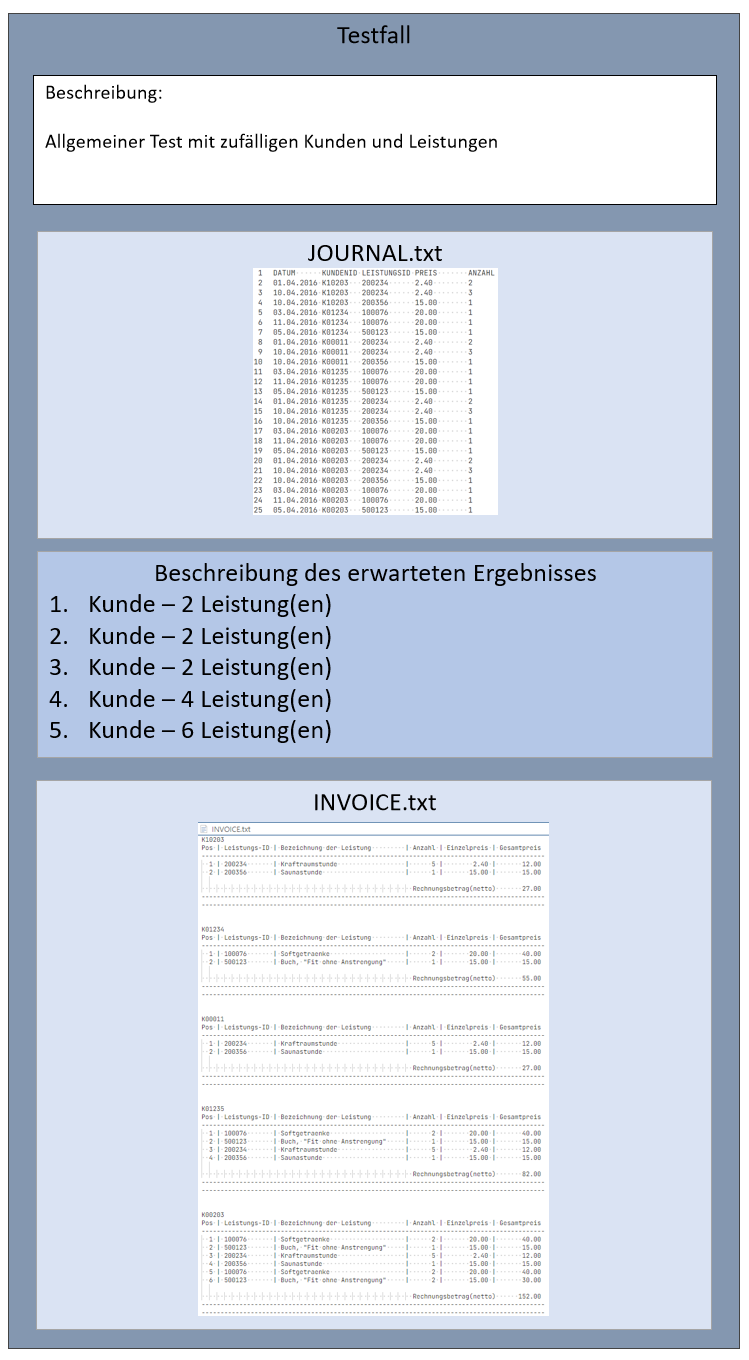
\includegraphics[width=\textwidth,height=\textheight,keepaspectratio]{images/Testdokumentation/Allgemeinfälle/fall_2.png}
    \caption{Allgemeiner Testfall 2}
\end{figure}

\begin{figure}[!h]
    \centering
    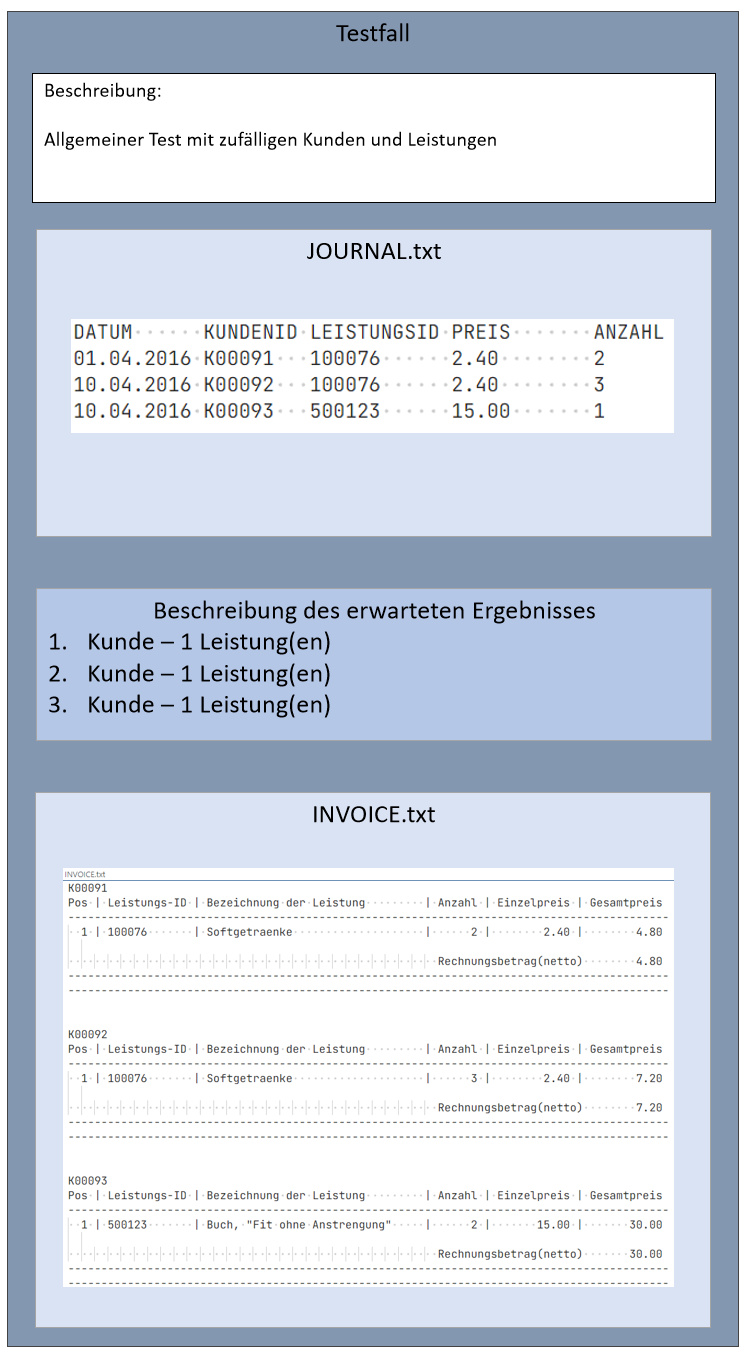
\includegraphics[width=\textwidth,height=\textheight,keepaspectratio]{images/Testdokumentation/Allgemeinfälle/fall_3.png}
    \caption{Allgemeiner Testfall 3}
\end{figure}

\section{Minimalfälle}\label{sec:minimalfaelle}
\begin{figure}[!h]
    \centering
    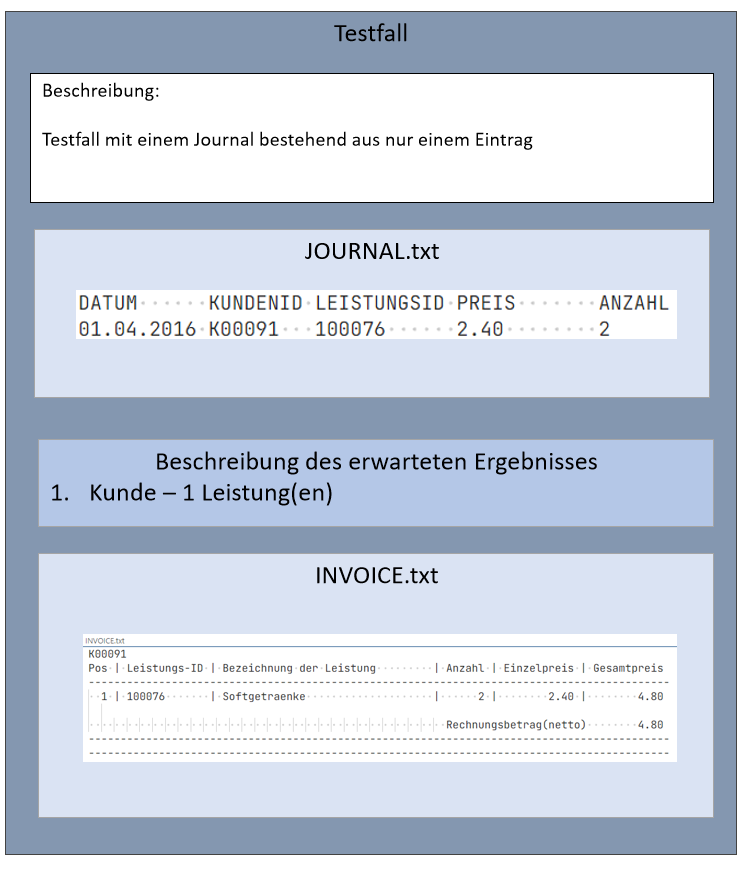
\includegraphics[width=\textwidth,height=\textheight,keepaspectratio]{images/Testdokumentation/Minimalfälle/1_eintrag.png}
    \caption{Journal mit nur einem Eintrag}
\end{figure}

\begin{figure}[!h]
    \centering
    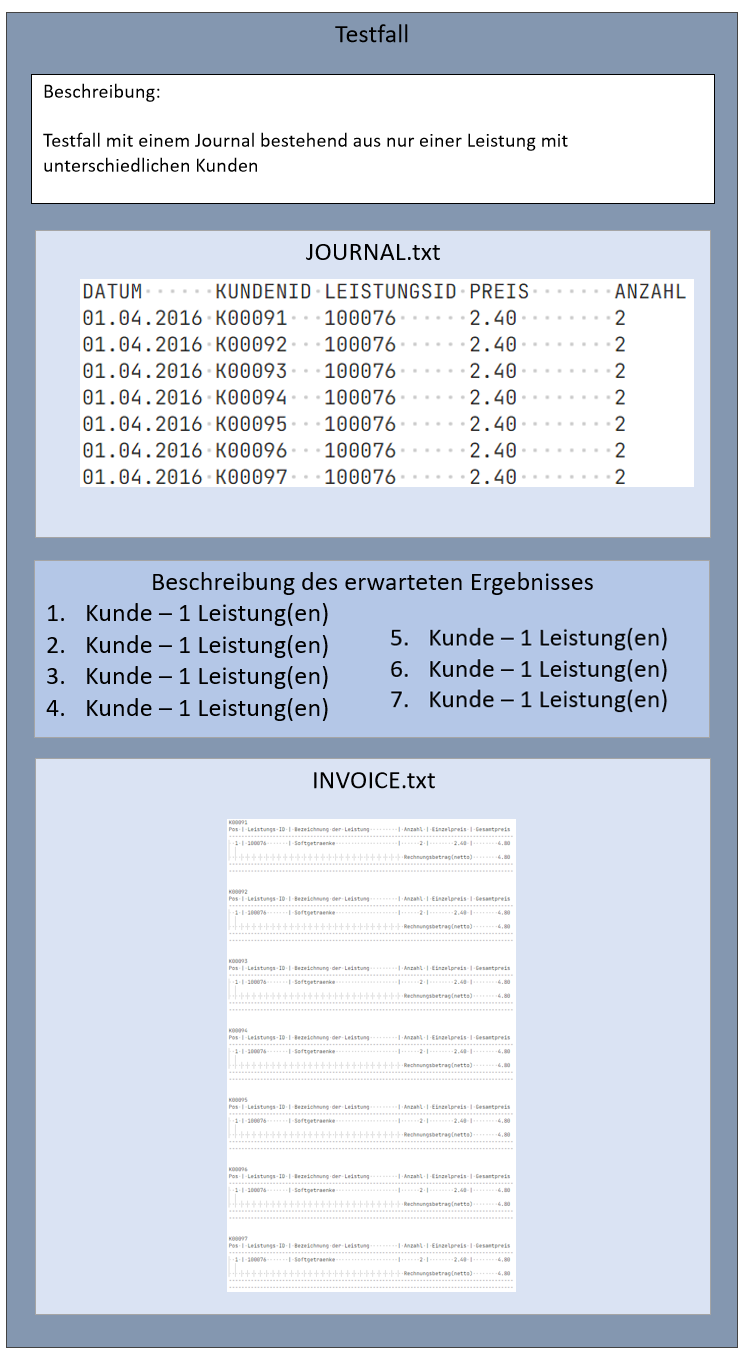
\includegraphics[width=\textwidth,height=\textheight,keepaspectratio]{images/Testdokumentation/Minimalfälle/1_kunde_verschiedene_leistungen.png}
    \caption{Journal mit nur einem einzigen Kunden}
\end{figure}

\begin{figure}[!h]
    \centering
    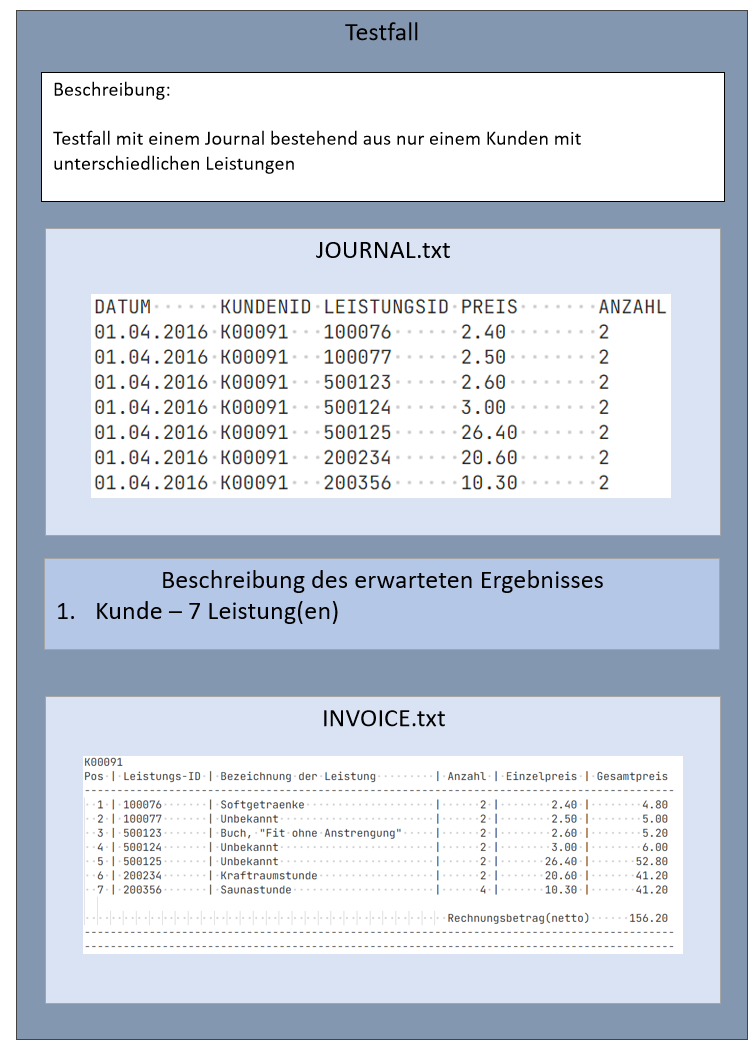
\includegraphics[width=\textwidth,height=\textheight,keepaspectratio]{images/Testdokumentation/Minimalfälle/verschiedene_kunden_1_leistung.png}
    \caption{Journal mit nur einer einzigen Leistung}
\end{figure}

\section{Sonderfälle}\label{sec:minimalfaelle}

\begin{figure}[!h]
    \centering
    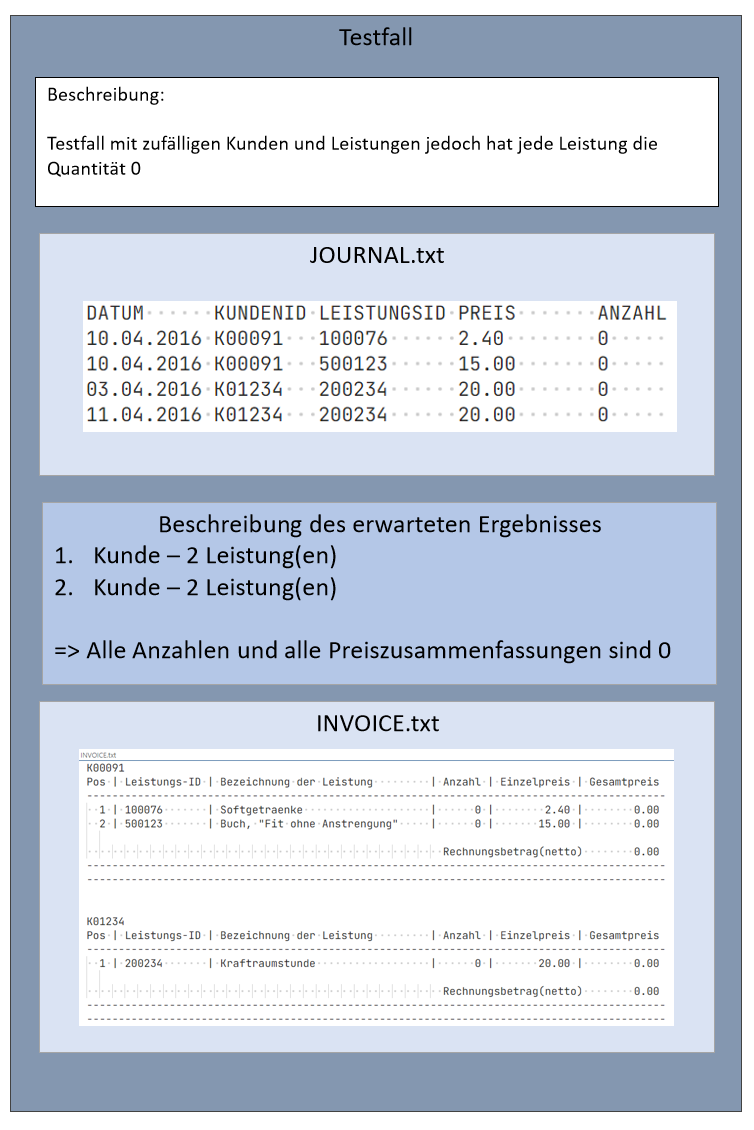
\includegraphics[width=\textwidth,height=\textheight,keepaspectratio]{images/Testdokumentation/Sonderfälle/anzahl_0.png}
    \caption{Alle Leistungen mit Anzahl 0}
\end{figure}

\begin{figure}[!h]
    \centering
    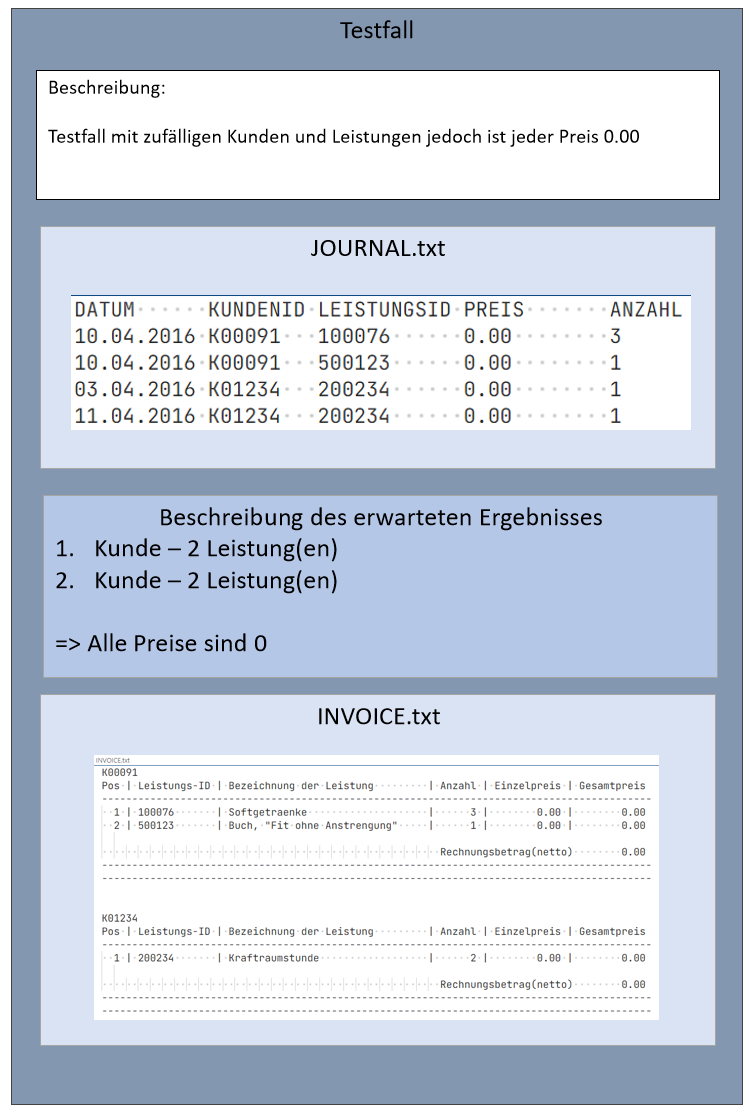
\includegraphics[width=\textwidth,height=\textheight,keepaspectratio]{images/Testdokumentation/Sonderfälle/preis_0.png}
    \caption{Alle Leistungen mit Preis 0.00}
\end{figure}

\begin{figure}[!h]
    \centering
    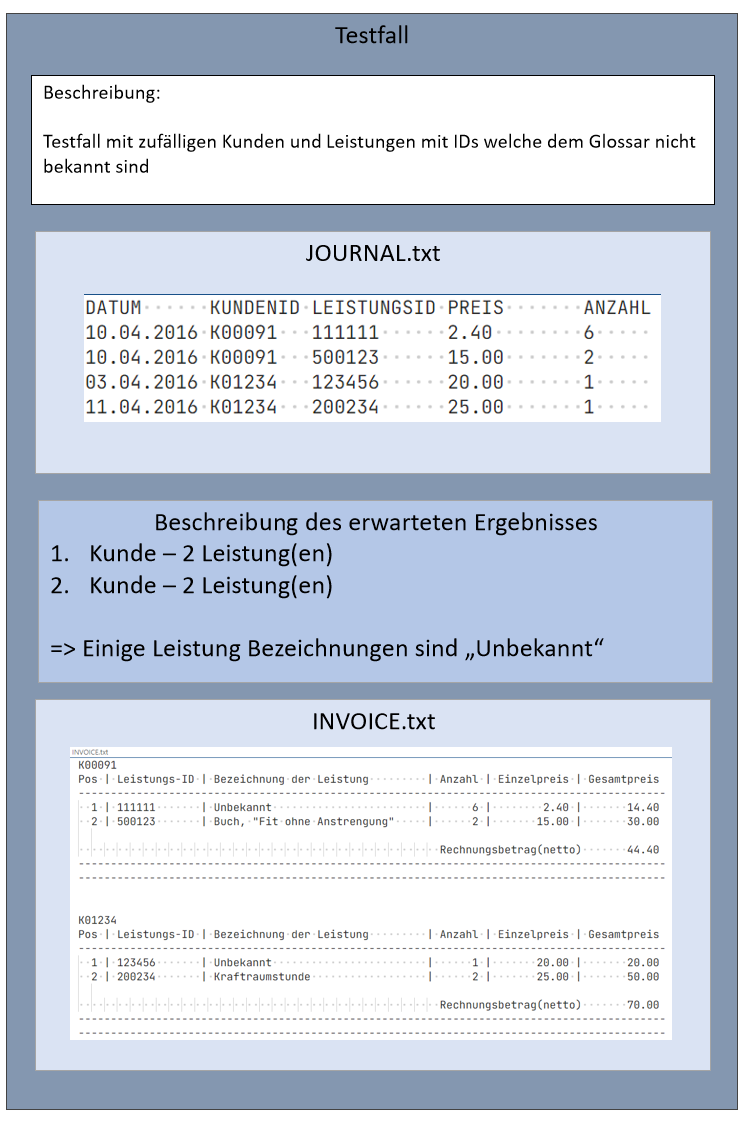
\includegraphics[width=\textwidth,height=\textheight,keepaspectratio]{images/Testdokumentation/Sonderfälle/unbekannte_leistung.png}
    \caption{Leistung-IDs sind teilweise nicht im Glossar vorhanden}
\end{figure}